\documentclass{article}


\usepackage{arxiv}

\usepackage[utf8]{inputenc} % allow utf-8 input
\usepackage[T1]{fontenc}    % use 8-bit T1 fonts
\usepackage{hyperref}       % hyperlinks
\usepackage{url}            % simple URL typesetting
\usepackage{booktabs}       % professional-quality tables
\usepackage{amsfonts}       % blackboard math symbols
\usepackage{nicefrac}       % compact symbols for 1/2, etc.
\usepackage{microtype}      % microtypography
\usepackage{lipsum}
\usepackage{graphicx}
\graphicspath{ {./images/} }


\title{Attention Phrenology: A spatial classification of attention heads}


\author{
 Giles Edkins \\
  Alignment Jam \#4 \\
  \texttt{} \\
   \And
 Keira Wiechecki \\
  Alignment Jam \#4 \\
  Department of Biology \\
  New York University \\
  \texttt{kaw504@nyu.edu} \\
}

\begin{document}
\maketitle
\begin{abstract}
Even with the same architecture, input, and tokens, the internal parameters of two language models can diverge substantially. However, they can nonetheless be made to converge on the same result. We attempt to determine whether heads with similar functions can be identified in different models. We present what we believe to be a novel method of language model interpretability analysis taking inspiration from biological imaging analysis.

\end{abstract}


% keywords can be removed
\keywords{Mechanistic Interpretability \and ML Safety \and Transformers}


\section{Introduction}

\section{Methods}
We trained 9 toy language models on [corpus]

We extracted weights from each head from each model in response to 1024 prompts. We used an autoencoder to compress the weights for each token pair 

\subsection{Giles Methods}
\subsubsection{Model Architecture}

9 models were trained. Each model was constructed using the **TransformerLens library. Each has the same architecture:
\begin{itemize}
	\item A single layer
	\item 8 Heads
	\item A context window of 16 tokens
	\item A model dimensionality of 256
	\item A head dimensionality of 64
	\item An MLP dimensionality of 2048
	\item A solu activation function
	\item The tokenizer taken from GPT-2
\end{itemize}

\subsubsection{Training}
Each model was trained for 4 epochs, with a sample of 30,000 datapoints (each 16 tokens long) taken from the **Brown corpus. An **AdamW optimizer was used, and a cross-entropy loss function.

\subsubsection{Attention weight extraction}
A sample of 1024 datapoints (each 16 tokens long) was taken from the Brown corpus. Each datapoint was fed through each model to calculate the logits, which were discarded - instead, we captured the attention pattern of each attention head. This was saved as a big CSV file.

\subsubsection{Head-distance matrix}
For each head of each model (72 total), we took all the attenion values and treated them as one long vector. Then we took the Euclidean distance between pairs of these vectors, to generate a 72x72 matrix.

\subsubsection{UMAP, TSNE and PCA visualizations}
We ran a 2-component Principal Component Analysis, UMAP and TSNE where the datapoints corresponded to the model-heads, and the features corresponded to attention weights on the different prompts. The projected components are shown, together with projections for 3 artificial points:

\begin{itemize}
	\item Each token only attending to itself
	\item Each token attending to all previous tokens equally
	\item Each token attending to itself and the previous token
\end{itemize}

\subsubsection{PCA components}
We ran a Principal Component Analysis where the datapoints corresponded to the model-heads, and the features corresponded to attention weights on the different prompts. The first 5 principal components, and the first 8 prompts, are shown.

\subsubsection{How much each token attends to the first token}
As a follow-up, we plotted a PCA projection of the attentions of various words in various prompts, against the first word only.

\subsubsection{Head knockout}
Here, further information was gathered from the models. In particular, we used the TransformerLens hook feature to erase the output from one of the heads on the given model, to investigate the effect of that head on the output. This allows, for a given prompt, producing a scatterplot of each token: the x-axis is the original logit values from the model, and the y-axis shows the logits when the head is knocked out.

The idea is that tokens above the diagonal are "suppressed" by the given head, and tokens below the diagonal are "promoted" by that head.

As a further investigation, we produced similar plots for each of the model-heads in one of the clusters, to see if they promote/suppress similar tokens.

\subsubsection{Head knockout with multiple prompts}
Finally, we took a selection of 64 prompts from the corpus and used the difference in probabilities (not logits) as a vector. Then we applied PCA dimensionality reduction to this and colored them according to the original clusters. The idea was to see whether clustering in the attention weights corresponds to clustering in the promoted/suppressed token space.


\section{Results}

\subsection{Giles Results}
\begin{figure}
    \centering
    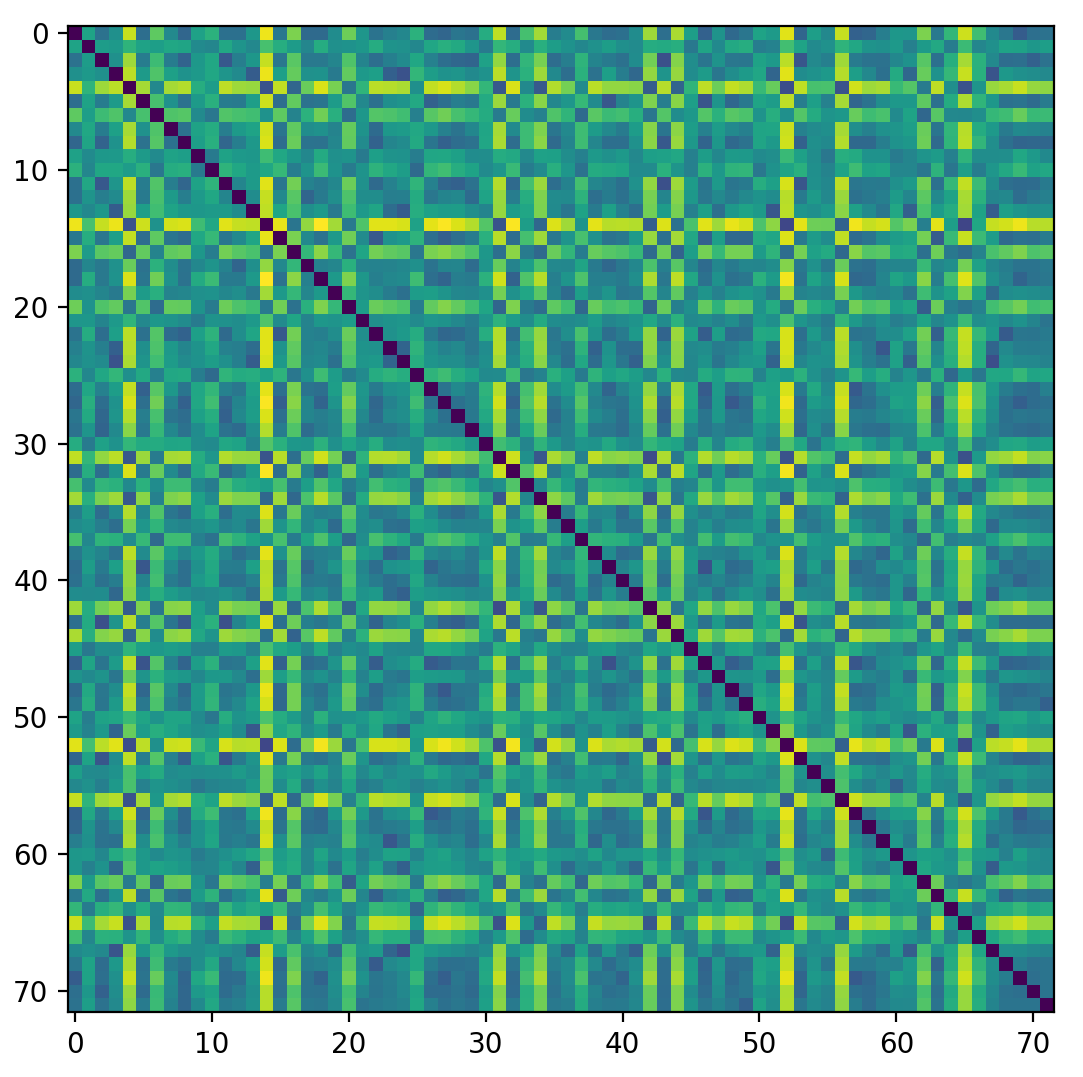
\includegraphics{images/head-distance-matrix.png}
\end{figure}

\begin{figure}
    \centering
    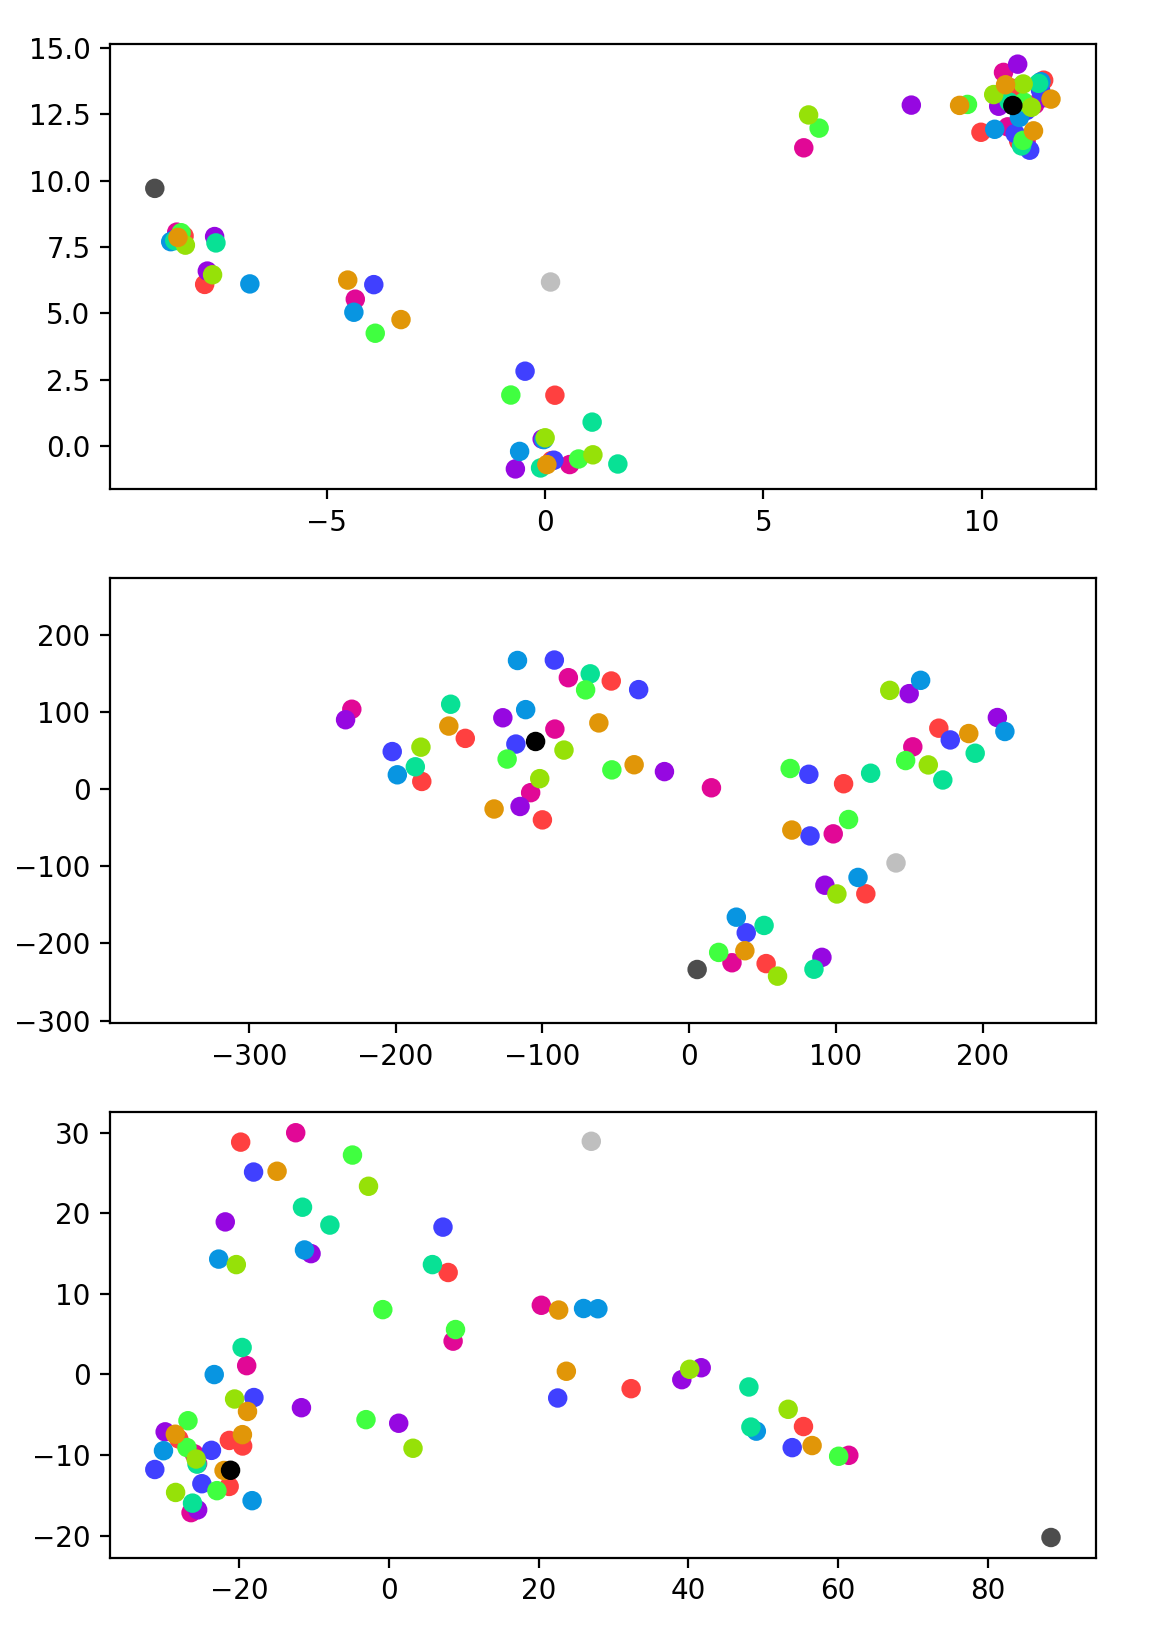
\includegraphics{images/umap-tsne-pca.png}
\end{figure}

\begin{figure}
    \centering
    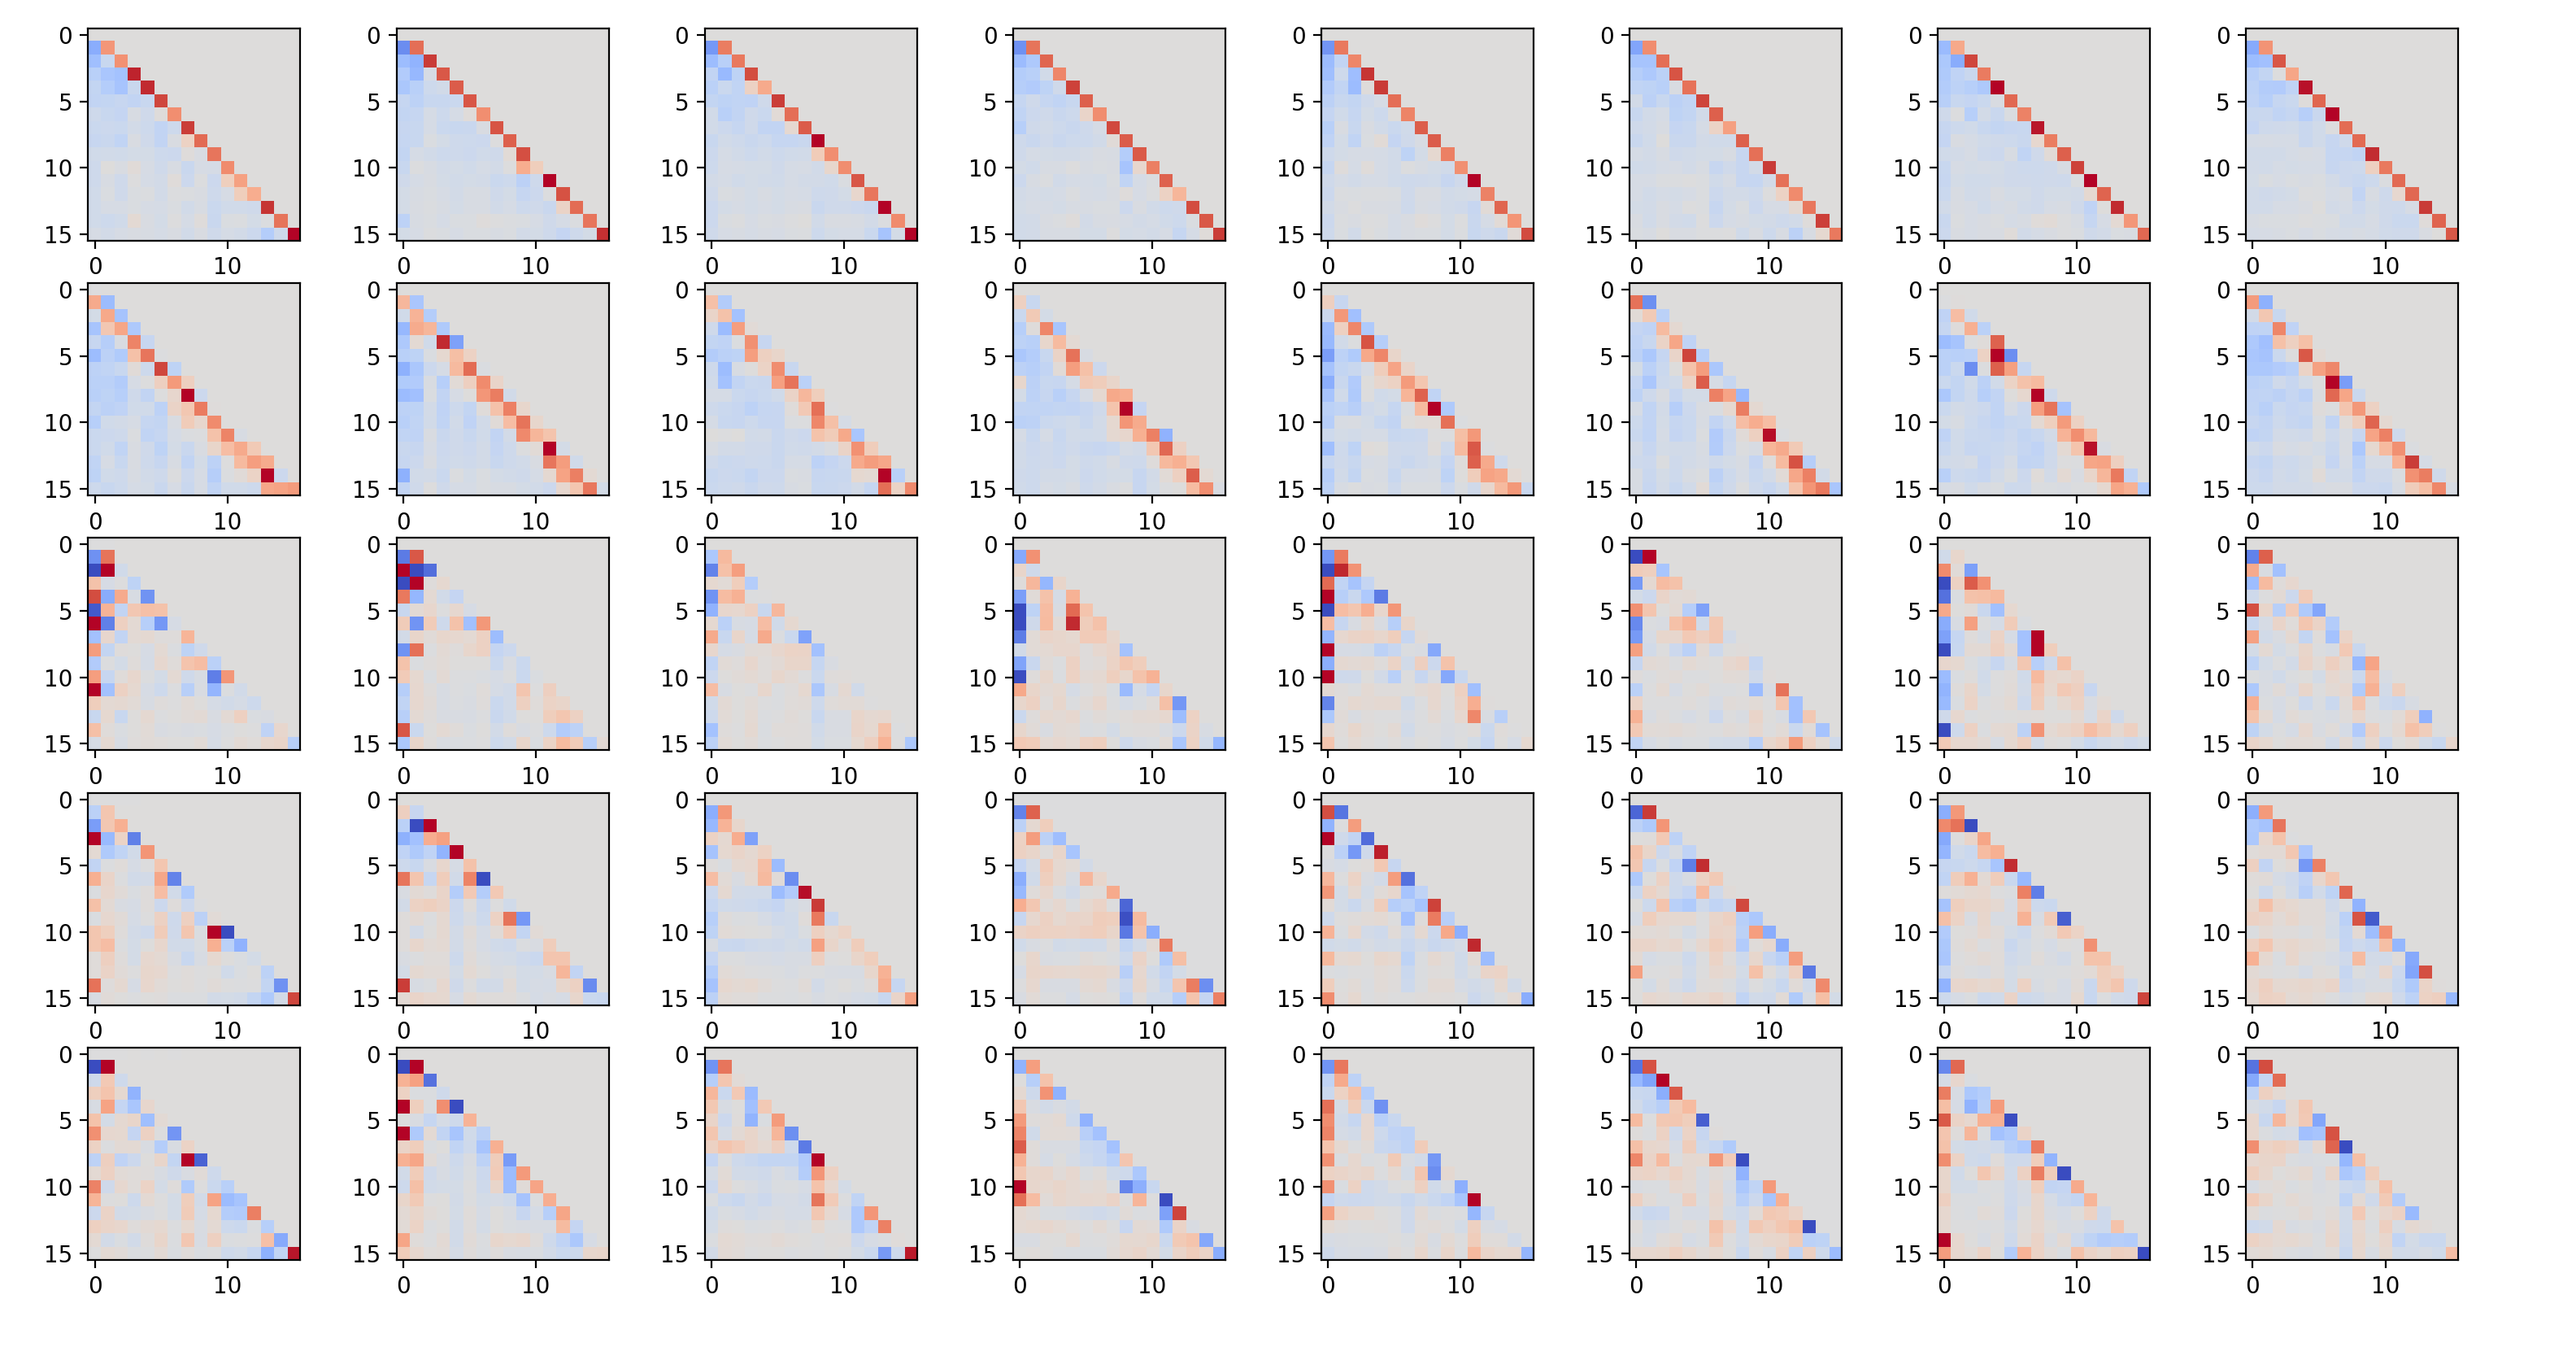
\includegraphics{images/pca-components.png}
\end{figure}

\begin{figure}
    \centering
    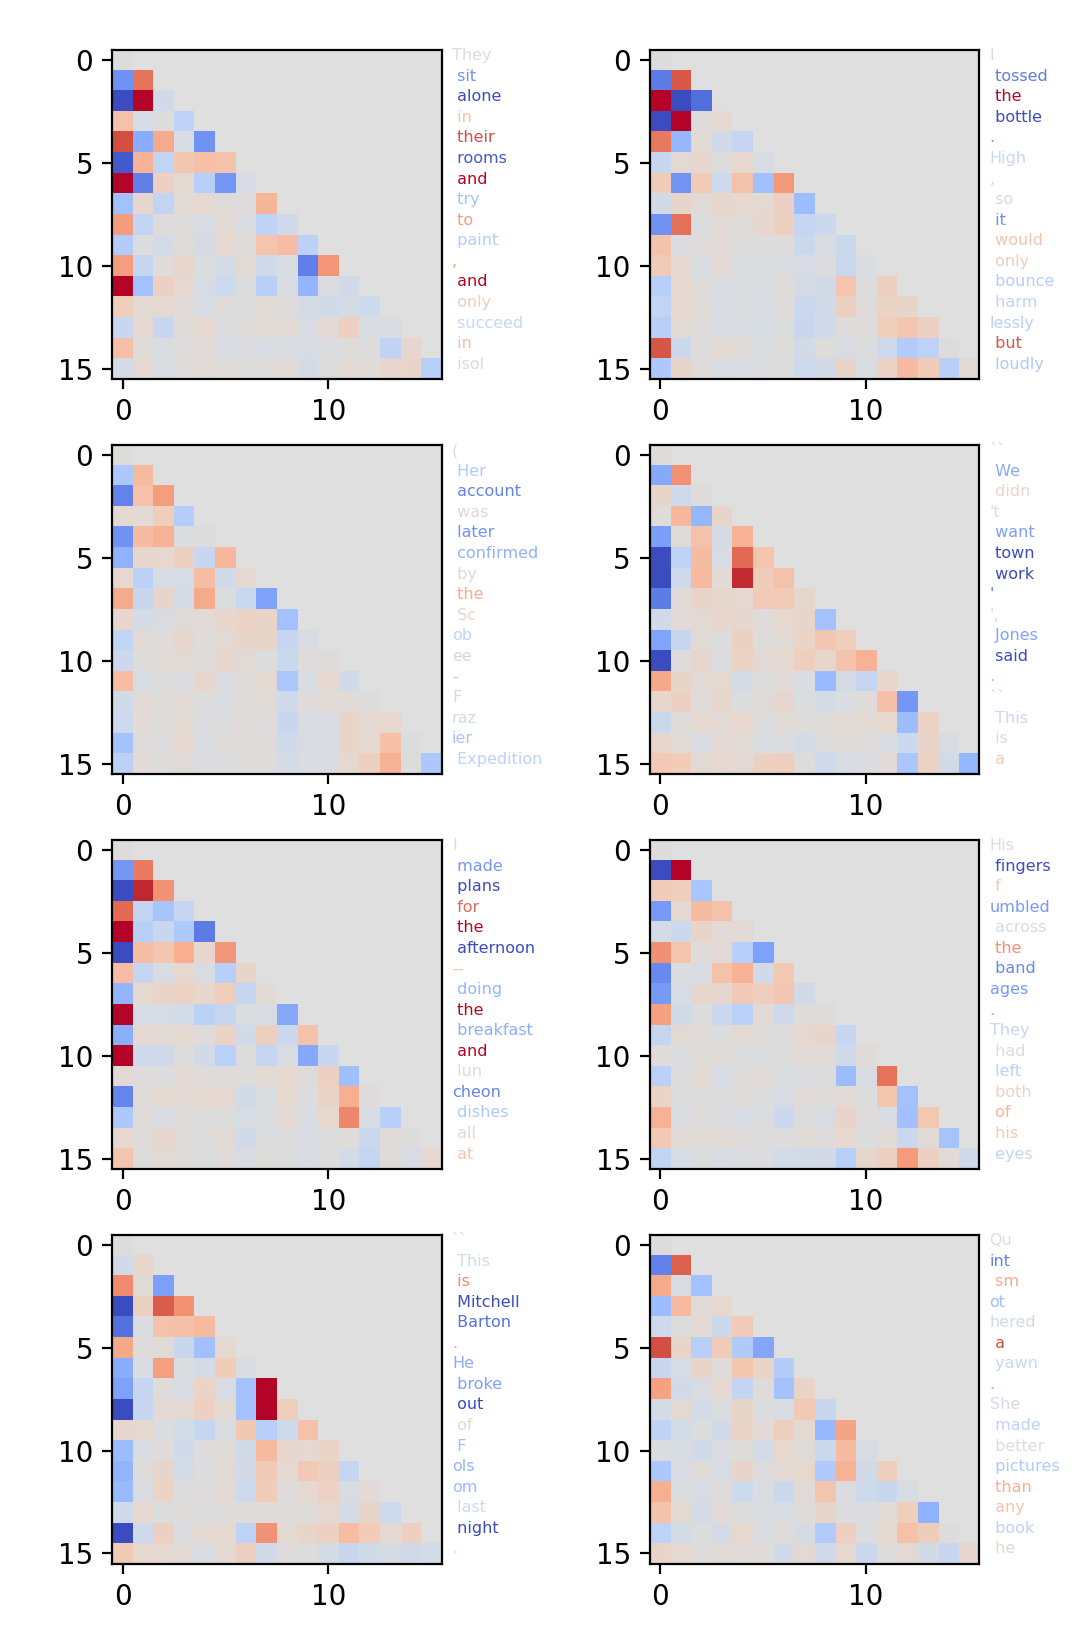
\includegraphics{images/pca-component-2.png}
\end{figure}

\begin{figure}
    \centering
    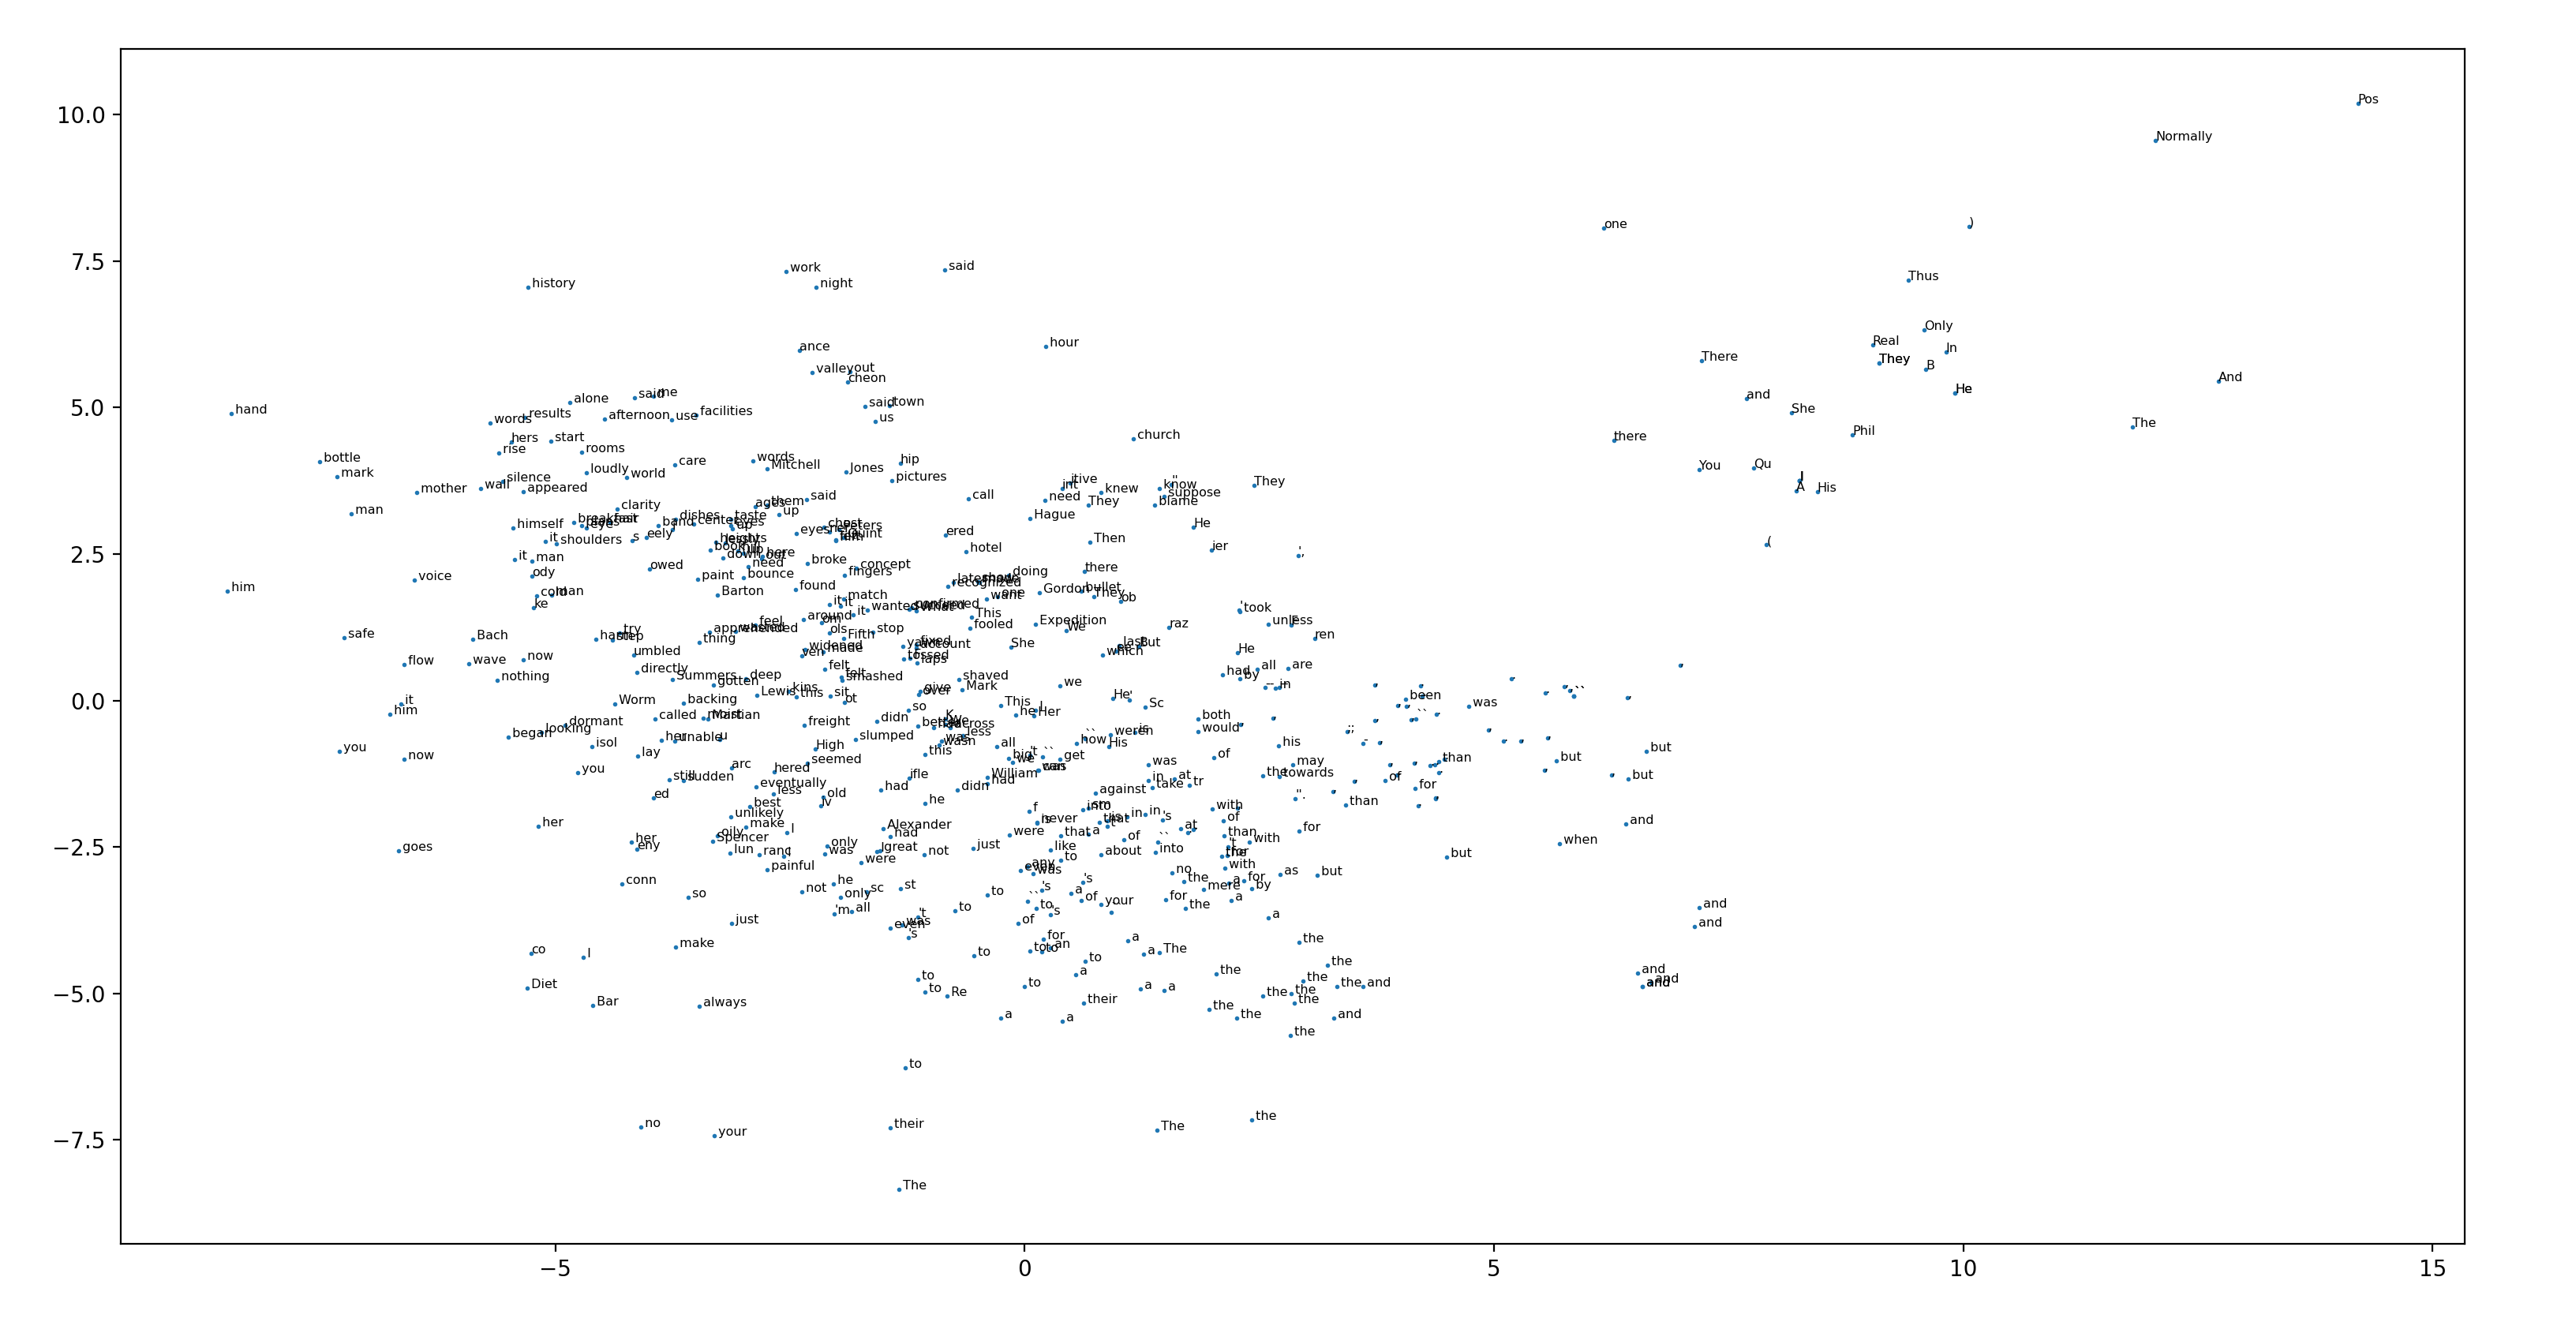
\includegraphics{images/attending-to-first-token.png}
\end{figure}

\begin{figure}
    \centering
    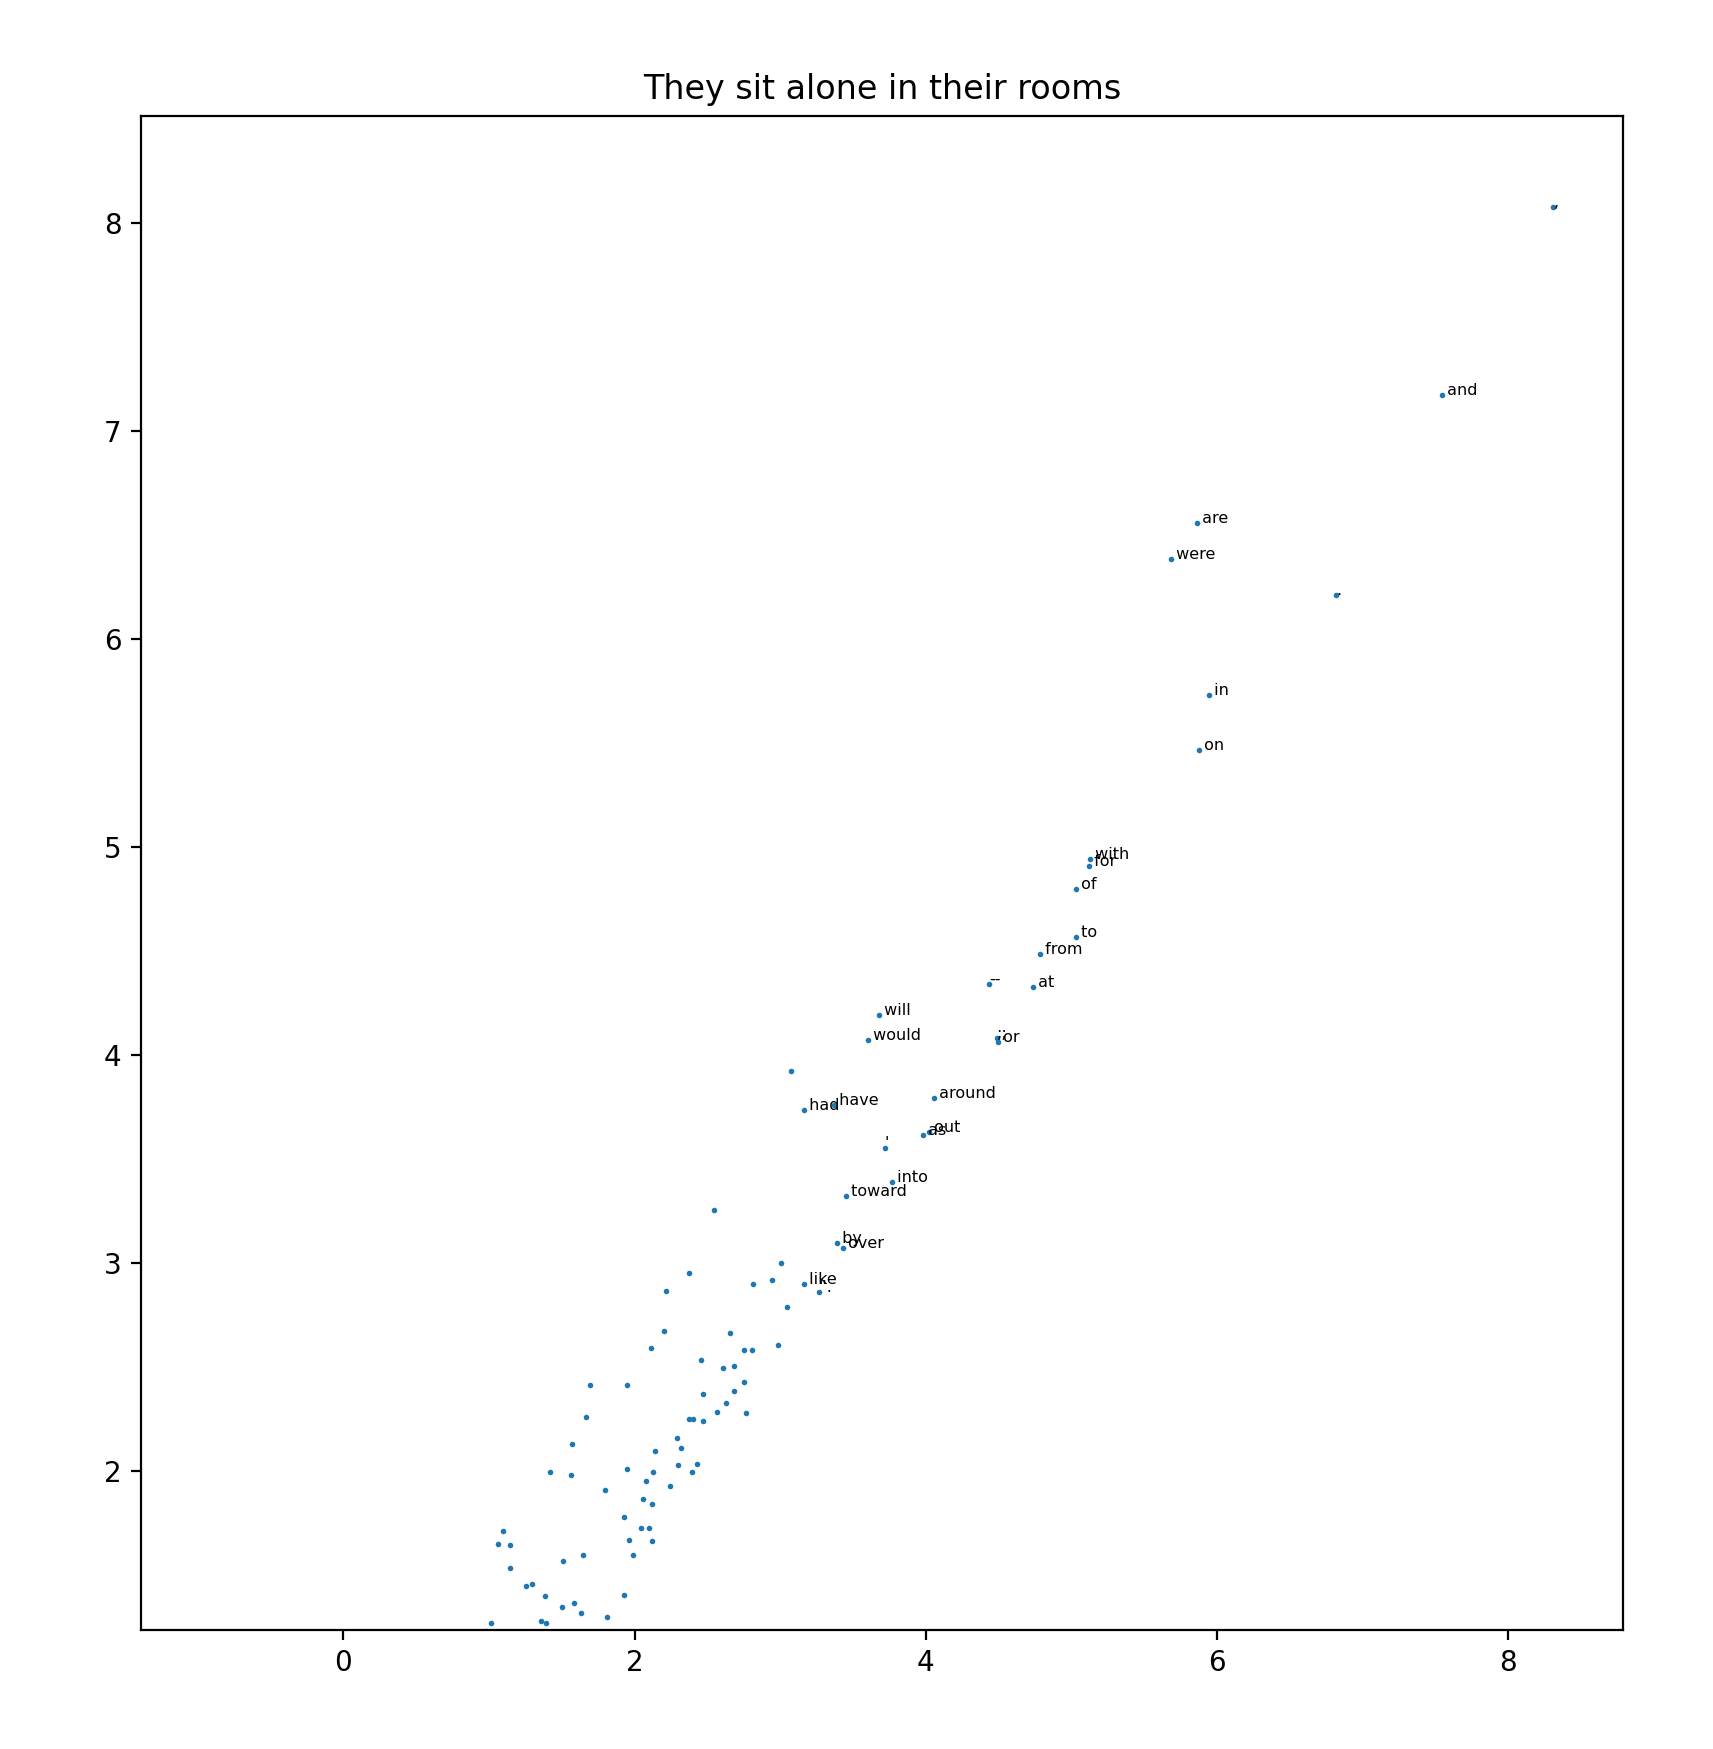
\includegraphics{images/knockout-one-prompt.png}
\end{figure}

\begin{figure}
    \centering
    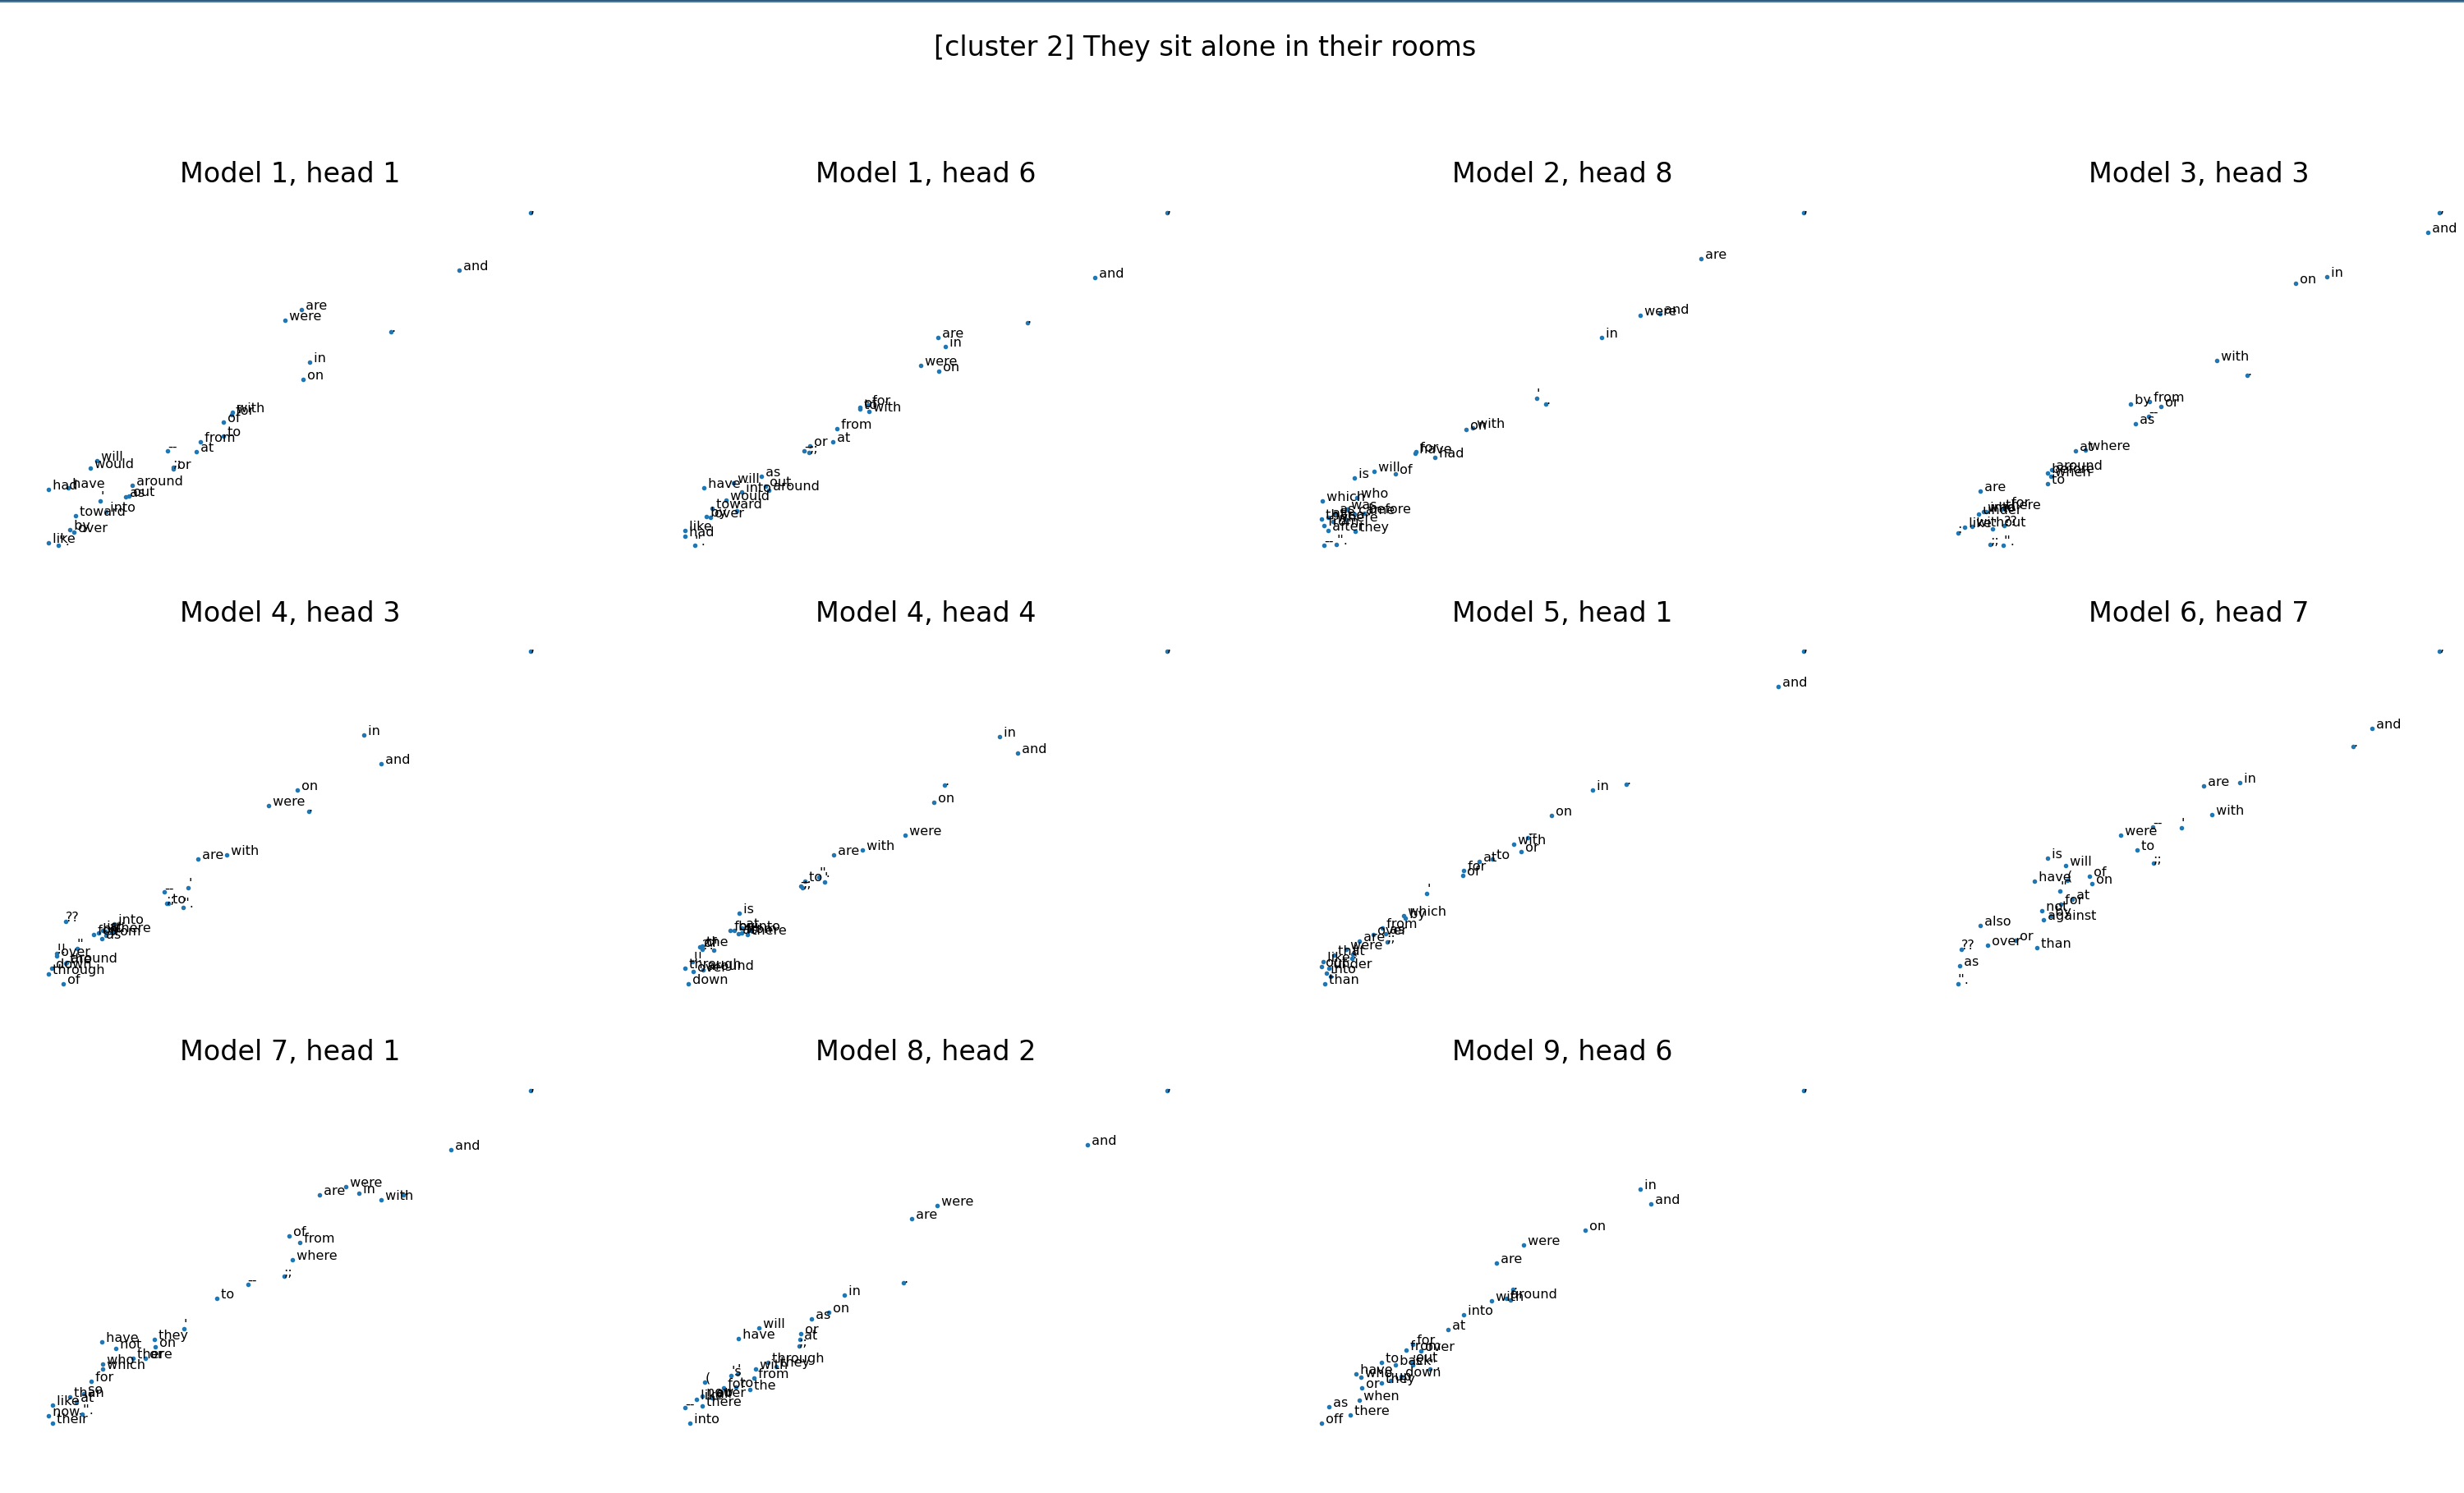
\includegraphics{images/knockout-one-prompt-many-models.png}
\end{figure}

\begin{figure}
    \centering
    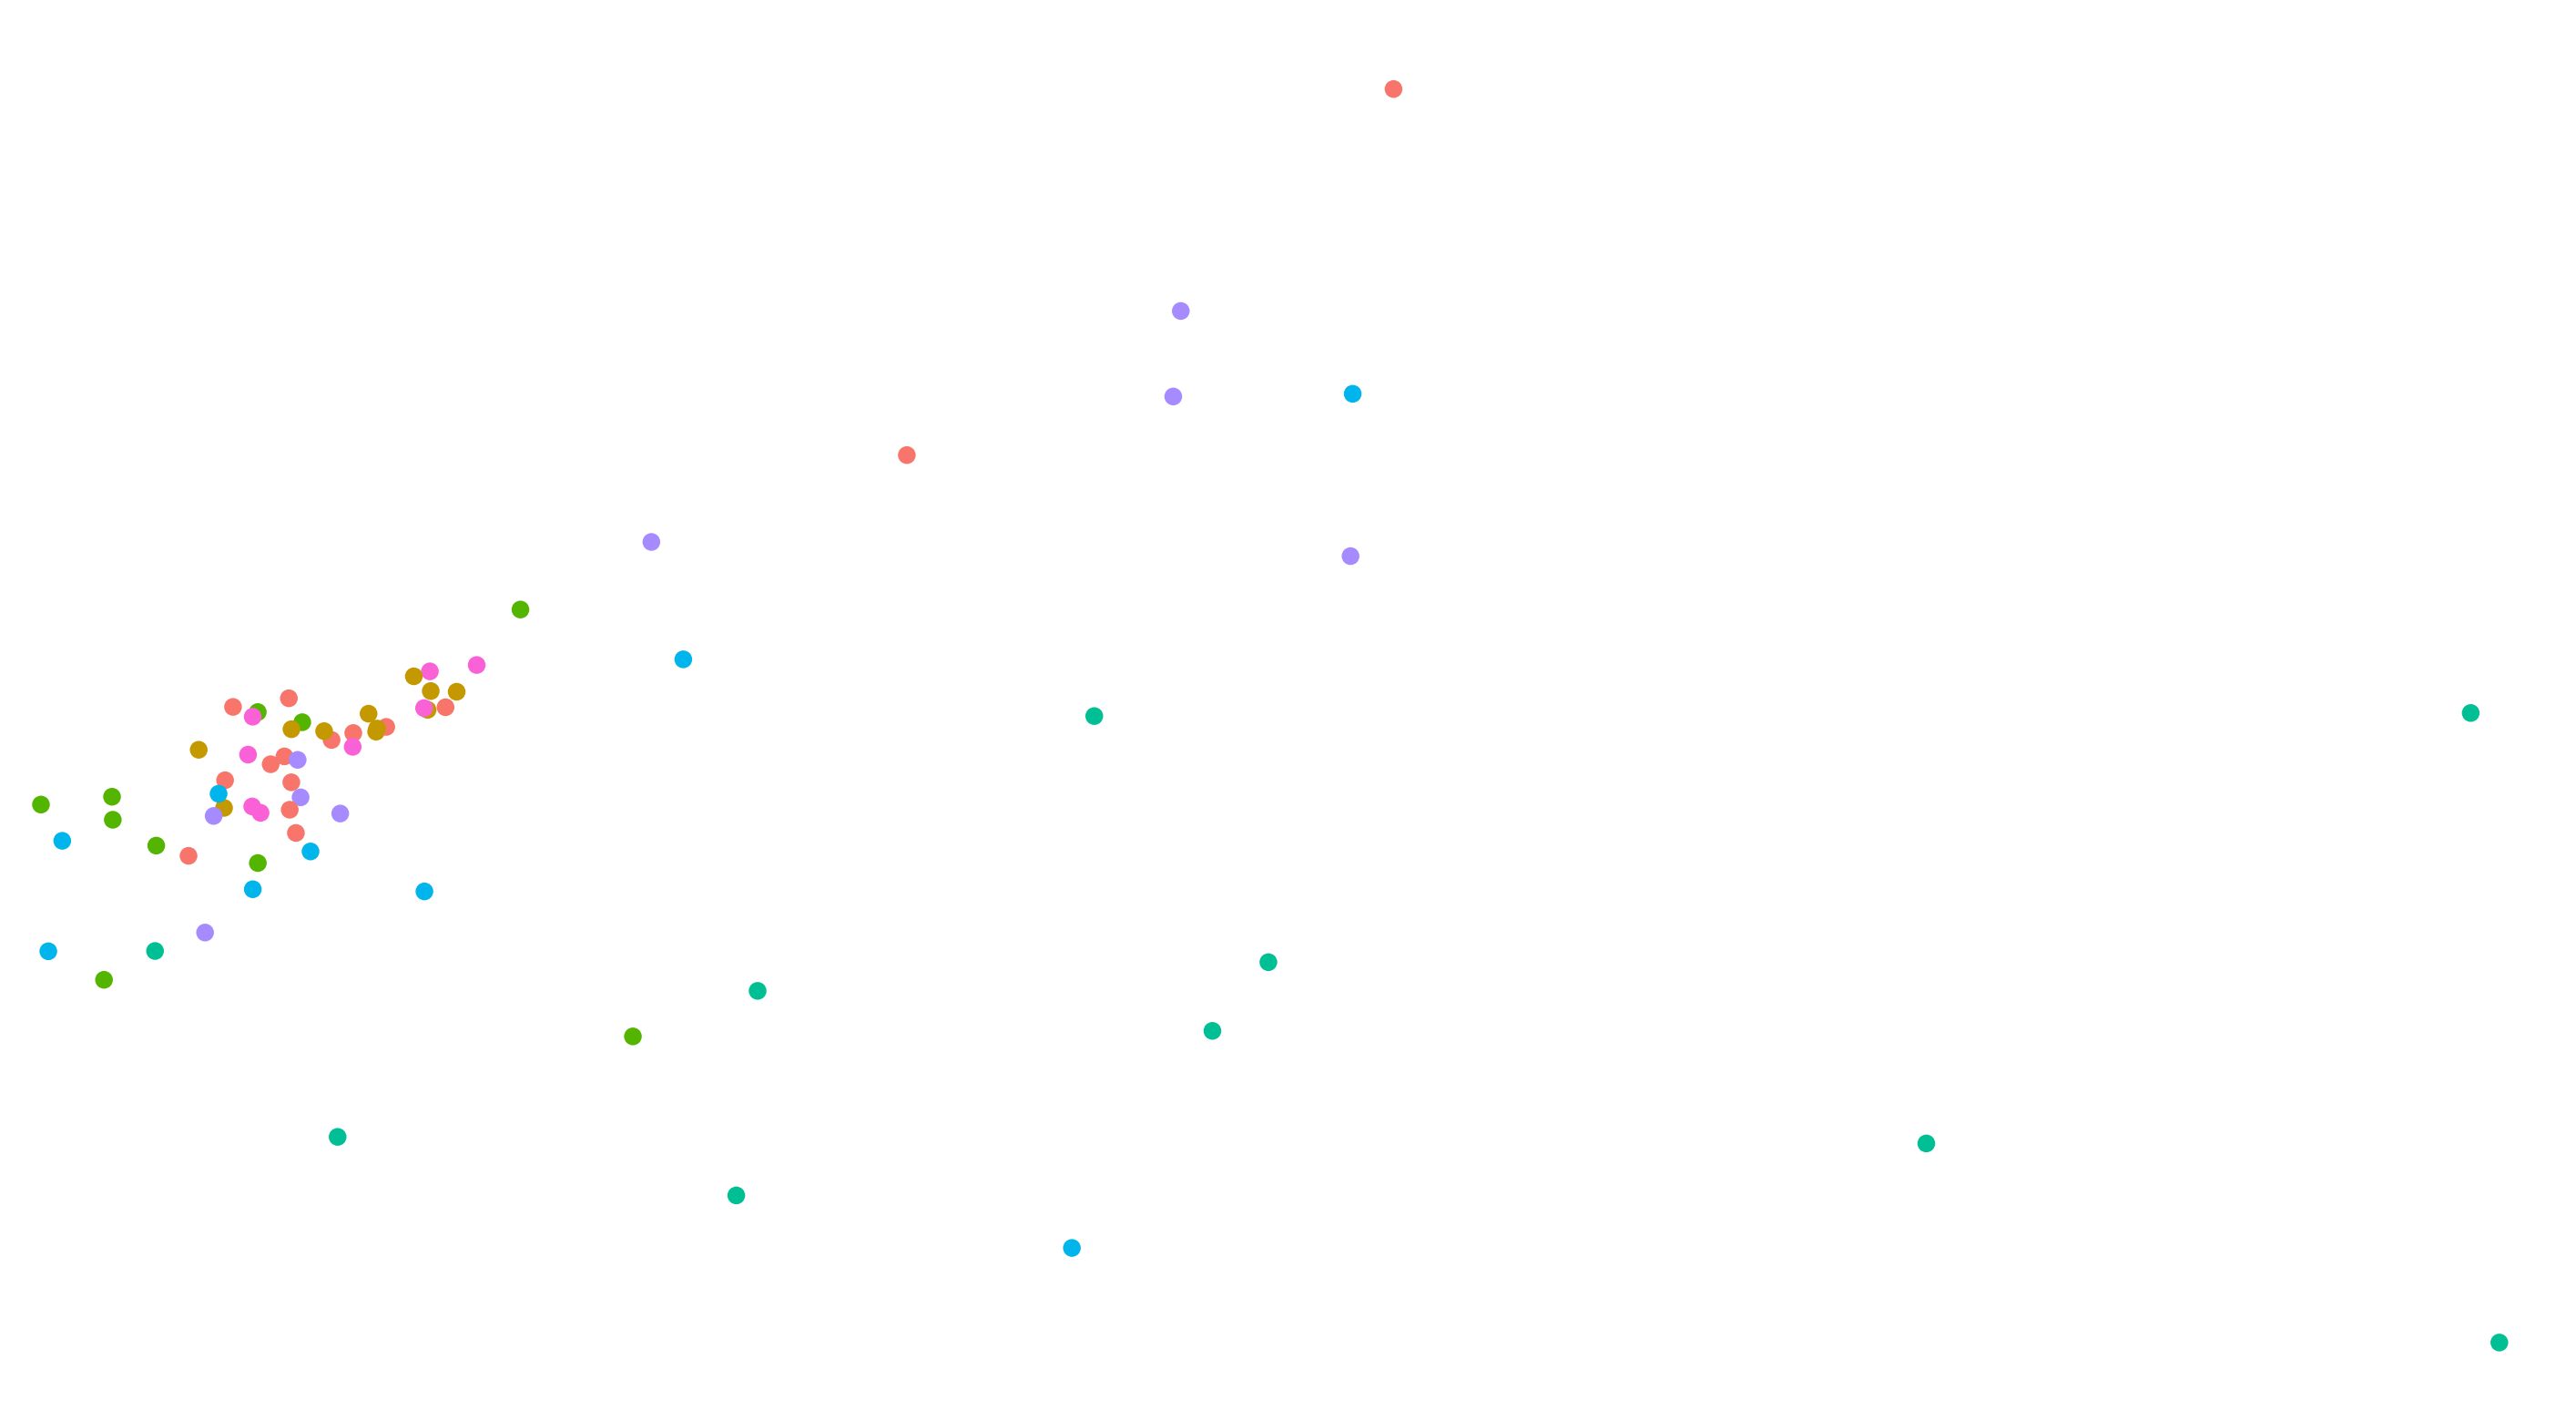
\includegraphics{images/knockout-64prompt.png}
\end{figure}

\section{Discussion}


\label{sec:others}
\lipsum[8] \cite{kour2014real,kour2014fast} and see \cite{hadash2018estimate}.

The documentation for \verb+natbib+ may be found at
\begin{center}
  \url{http://mirrors.ctan.org/macros/latex/contrib/natbib/natnotes.pdf}
\end{center}
Of note is the command \verb+\citet+, which produces citations
appropriate for use in inline text.  For example,
\begin{verbatim}
   \citet{hasselmo} investigated\dots
\end{verbatim}
produces
\begin{quote}
  Hasselmo, et al.\ (1995) investigated\dots
\end{quote}

\begin{center}
  \url{https://www.ctan.org/pkg/booktabs}
\end{center}


\subsection{Figures}
\lipsum[10] 
See Figure \ref{fig:fig1}. Here is how you add footnotes. \footnote{Sample of the first footnote.}
\lipsum[11] 

\begin{figure}
  \centering
  \fbox{\rule[-.5cm]{4cm}{4cm} \rule[-.5cm]{4cm}{0cm}}
  \caption{Sample figure caption.}
  \label{fig:fig1}
\end{figure}

\begin{figure} % picture
    \centering
    \includegraphics{test.png}
\end{figure}

\subsection{Tables}
\lipsum[12]
See awesome Table~\ref{tab:table}.

\begin{table}
 \caption{Sample table title}
  \centering
  \begin{tabular}{lll}
    \toprule
    \multicolumn{2}{c}{Part}                   \\
    \cmidrule(r){1-2}
    Name     & Description     & Size ($\mu$m) \\
    \midrule
    Dendrite & Input terminal  & $\sim$100     \\
    Axon     & Output terminal & $\sim$10      \\
    Soma     & Cell body       & up to $10^6$  \\
    \bottomrule
  \end{tabular}
  \label{tab:table}
\end{table}

\subsection{Lists}
\begin{itemize}
\item Lorem ipsum dolor sit amet
\item consectetur adipiscing elit. 
\item Aliquam dignissim blandit est, in dictum tortor gravida eget. In ac rutrum magna.
\end{itemize}


\bibliographystyle{unsrt}  
%\bibliography{references}  %%% Remove comment to use the external .bib file (using bibtex).
%%% and comment out the ``thebibliography'' section.


%%% Comment out this section when you \bibliography{references} is enabled.
\begin{thebibliography}{1}

\bibitem{kour2014real}
George Kour and Raid Saabne.
\newblock Real-time segmentation of on-line handwritten arabic script.
\newblock In {\em Frontiers in Handwriting Recognition (ICFHR), 2014 14th
  International Conference on}, pages 417--422. IEEE, 2014.

\bibitem{kour2014fast}
George Kour and Raid Saabne.
\newblock Fast classification of handwritten on-line arabic characters.
\newblock In {\em Soft Computing and Pattern Recognition (SoCPaR), 2014 6th
  International Conference of}, pages 312--318. IEEE, 2014.

\bibitem{hadash2018estimate}
Guy Hadash, Einat Kermany, Boaz Carmeli, Ofer Lavi, George Kour, and Alon
  Jacovi.
\newblock Estimate and replace: A novel approach to integrating deep neural
  networks with existing applications.
\newblock {\em arXiv preprint arXiv:1804.09028}, 2018.

\end{thebibliography}


\end{document}


